\documentclass[pdftex,francais]{beamer}

% Copyright 2004 by Till Tantau <tantau@users.sourceforge.net>.
%
% This file can be redistributed and/or modified under
% the terms of the GNU Public License, version 2.

%% \ifx\themename\undefined
%%   \def\themename{default}
%% \fi

\usetheme{lama}
%\usetheme{Madrid}
%\usecolortheme{crane}

\usepackage{multirow}
\usepackage[latin1]{inputenc}           %%%  
\usepackage[T1]{fontenc}                %%%
\usepackage[francais]{babel}            %%%

\usepackage{multimedia}
\usepackage{hyperref}
\usepackage{tikz}
\usepackage{listings}

%\newtheorem{theorem}{Th�or�me}

%\setbeamercovered{transparent}

\title[DGtal topology module]{DGtal: Topology module\\
     \url{http://liris.cnrs.fr/dgtal}
}

\author[J.-O. Lachaud]{Jacques-Olivier Lachaud}

\date{DGtal Meeting, September 2011}


\graphicspath{{Figures/},{Images/},{Graphs/}}

%%% \AtBeginSection[]
%%% {
%%%   \begin{frame}<beamer>
%%%     \frametitle{Plan}
%%%     \tableofcontents[currentsection] %,currentsubsection]
%%%   \end{frame}
%%% }


\renewcommand{\vec}[1]{\mathbf{#1}}

% space of the real numbers
\newcommand{\R}{\ensuremath{\mathbb{R}}}
% space of the integer numbers
\newcommand{\Z}{\ensuremath{\mathbb{Z}}}
% Digitization process of step h (1)
\newcommand{\Dig}[1]{\ensuremath{\mathrm{Dig}_{#1}}}
% Family of shape
\newcommand{\SF}[0]{\ensuremath{\mathbb{F}}}
% Topological boundary of X (1).
\newcommand{\TB}[1]{\ensuremath{\partial #1}}
% Discrete geometric estimator of G (1)
\newcommand{\DGE}[1]{\ensuremath{E_{#1}}}
% Reference shape of digital object O (1) with grid step $h$ (2).
\newcommand{\RS}[2]{\ensuremath{R_{#1,#2}}}

% Digital contour.
\newcommand{\DC}{\ensuremath{C}}
% Continuous contour.
\newcommand{\CC}{\ensuremath{\mathcal{C}}}
% A point indexed by i (1) on the digital contour.
\newcommand{\PT}[1]{\ensuremath{\DC_{#1}}}
% A sequence of points indexed by i (1) on the digital contour.
\newcommand{\PTS}[2]{\ensuremath{\DC_{#1,#2}}}
% Predicate stating that the digital curve is a segment between indices 1 and 2
\newcommand{\SPRED}[2]{\ensuremath{S(#1,#2)}}
% ET logique
\newcommand{\AND}[0]{\ensuremath{\wedge}}
% OU logique
\newcommand{\OR}[0]{\ensuremath{\vee}}

% Tangent direction mapping of curve C (1)
\newcommand{\TGT}[1]{\ensuremath{\theta_{#1}}}
% Integral of squared curvature of curve C (1)
\newcommand{\ISC}[1]{\ensuremath{J[#1]}}
% Smallest possible tangent direction at constraint l (1)
\newcommand{\MinTD}[1]{\ensuremath{a_{#1}}}
% Largest possible tangent direction at constraint l (1)
\newcommand{\MaxTD}[1]{\ensuremath{b_{#1}}}
% Unknown tangent direction at constraint l (1)
\newcommand{\UnkTD}[1]{\ensuremath{t_{#1}}}

% ideal multiscale criterion
\newcommand{\IMSC}[2]{\ensuremath{\mu_{#1}(#2)}}
% multiscale profile
\newcommand{\MSP}[2]{\ensuremath{\mathcal{P}_{#1}(#2)}}
% threshold flat/curve
\newcommand{\CThreshold}[0]{\ensuremath{t_{f/c}}}
% threshold noise
\newcommand{\NThreshold}[0]{\ensuremath{t_{m}}}
% noise level
\newcommand{\NL}[0]{\ensuremath{\nu}}
% slope linear regression 
\newcommand{\SLR}[2]{\ensuremath{\theta_{#1}}}





% Pencil of maximal segments around a point.
\newcommand{\PE}[1]{\ensuremath{{\mathcal P}(#1)}}
% Tangent orientation of the maximal segment.
\newcommand{\TO}[1]{\ensuremath{\theta_#1}}
% lambda function for interpolation.
\newcommand{\LF}{\ensuremath{\lambda}}
% \lambda-MS tangent orientation.
\newcommand{\LTO}[1]{\ensuremath{\hat{\theta}(#1)}}
% \lambda-MS tangent orientation variation.
\newcommand{\LTOP}[1]{\ensuremath{\hat{\theta}'(#1)}}

%\definecolor{rougeSW_}{rgb}{0.968627,0.011765,0.015686}
\definecolor{darkgreen}{rgb}{0.0,0.6,0.0}
\definecolor{lightblue}{rgb}{0.5,0.5,1.0}
\definecolor{magenta}{rgb}{1.0,0.0,1.0}
\newcommand{\alertred}[1]{{\color{red}#1}}
\newcommand{\Cb}[1]{{\color{blue}#1}}
\newcommand{\Cdg}[1]{{\color{darkgreen}#1}}
\newcommand{\textmagenta}[1]{{\color{magenta}#1}}
\newcommand{\Implies}{{\ensuremath{\Rightarrow}}}

\newcommand{\Refs}[1]{{\color{lightblue}#1}}
\newcommand{\Cite}[1]{\Refs{[#1]}}
\newcommand{\Etal}{{\em et al.}}
\newtheorem{remark}{Remarque}
% Digitization process of step h (1)
\newcommand{\DigGh}[2]{\ensuremath{\mathrm{Dig}_{#2}(#1)}}
\newcommand{\BigT}{\ensuremath{\Theta}}
\newcommand{\BigO}{\ensuremath{O}}

\newcommand{\TAN}[0]{\ensuremath{\theta}}
% Position estimator
\newcommand{\EPOS}[0]{\ensuremath{\hat{{x}}}}
% Convexity Position estimator 
\newcommand{\ECONVPOS}[0]{\ensuremath{\hat{x}^\mathrm{conv}}}
% tangent estimator base MS.
\newcommand{\ETANMS}[0]{\ensuremath{\hat{\TAN}^{\text{MS}}}}
% tangent estimator base arete du CDP.
\newcommand{\ETANEDGE}[0]{\ensuremath{\hat{\TAN}^{\text{conv}}}}
% estimateur de longueur elementaire d'un surfel (1) sur le bord discretise de X(2) de pas h(3).

\newcommand{\Class}[1]{\alert{\texttt{#1}}}
\newcommand{\Concept}[1]{\texttt{\color{magenta}#1}}
\newcommand{\Method}[1]{\texttt{\color{lightblue}#1}}


\setbeamercolor{qcolorb}{fg={blue!20!black},bg={blue!15!white}}
\setbeamercolor{qcolorub}{fg={blue!10!black},bg={blue!30!white}}
\setbeamercolor{qcolorlb}{fg={blue!20!black},bg={blue!8!white}}
\setbeamercolor{qcolorulb}{fg={blue!10!black},bg={blue!40!white}}
\setbeamercolor{qcolorg}{fg={green!20!black},bg={green!15!white}}
\setbeamercolor{qcolorug}{fg={green!10!black},bg={green!30!white}}
\setbeamercolor{qcolorlg}{fg={green!20!black},bg={green!8!white}}
\setbeamercolor{qcolorulg}{fg={green!10!black},bg={green!40!white}}
\setbeamercolor{qcolorr}{fg={red!20!black},bg={red!15!white}}
\setbeamercolor{qcolorur}{fg={red!10!black},bg={red!30!white}}
\setbeamercolor{qcolorlr}{fg={red!20!black},bg={red!8!white}}
\setbeamercolor{qcolorulr}{fg={red!10!black},bg={red!40!white}}
\newenvironment{myblockbluish}[2]%
	       {\begin{beamerboxesrounded}[lower=qcolorb,upper=qcolorub,width=#1,shadow=true]{#2}}{\end{beamerboxesrounded}}
\newenvironment{myblocklbluish}[2]%
	       {\begin{beamerboxesrounded}[lower=qcolorlb,upper=qcolorulb,width=#1,shadow=true]{#2}}{\end{beamerboxesrounded}}
\newenvironment{myblockgreenish}[2]%
	       {\begin{beamerboxesrounded}[lower=qcolorg,upper=qcolorug,width=#1,shadow=true]{#2}}{\end{beamerboxesrounded}}
\newenvironment{myblocklgreenish}[2]%
	       {\begin{beamerboxesrounded}[lower=qcolorlg,upper=qcolorulg,width=#1,shadow=true]{#2}}{\end{beamerboxesrounded}}
\newenvironment{myblockredish}[2]%
	       {\begin{beamerboxesrounded}[lower=qcolorr,upper=qcolorur,width=#1
,shadow=true]{#2}}{\end{beamerboxesrounded}}
\newenvironment{myblocklredish}[2]%
	       {\begin{beamerboxesrounded}[lower=qcolorlr,upper=qcolorulr,width=#1,shadow=true]{#2}}{\end{beamerboxesrounded}}

%%%%%%%%%%%%%%%%%%%%%%%%%%%%%%%%%%%%%%%%%%%%%%%%%%%%%%%%%%%%%%%%%%%%%%%%%%%%%%%
%%%%%%%%%%%%%%%%%%%%%%%%%%%%%%%%%%%%%%%%%%%%%%%%%%%%%%%%%%%%%%%%%%%%%%%%%%%%%%%
%%%%%%%%%%%%%%%%%%%%%%%%%%%%%%%%%%%%%%%%%%%%%%%%%%%%%%%%%%%%%%%%%%%%%%%%%%%%%%%
\begin{document}

\newlength{\unquart}
\setlength{\unquart}{0.21\textwidth}

%------------------------------------------------------------------------------
\begin{frame}
  \titlepage
\end{frame}
%------------------------------------------------------------------------------

\section{Package topology}

%------------------------------------------------------------------------------
\begin{frame}[squeeze]%[allowframebreaks]
  \frametitle{Package description}

  \begin{myblocklbluish}{\textwidth}{Should contain}
    \begin{itemize}
      \small
    \item classical digital topology {\em � la} Rosenfeld
    \item cartesian cellular topology
    \item digital surface topology {\em � la} Herman
    \item must be the base block of geometric algorithms
    \end{itemize}
  \end{myblocklbluish}
  \begin{myblocklgreenish}{\textwidth}{Examples}
    \begin{itemize}
      \small
    \item adjacencies, connected components, simple points, thinning
    \item cells, boundary operators, incidence, opening, closing
    \item contours, surfel adjacency, surface tracking
    \item topological invariants
    \end{itemize}
  \end{myblocklgreenish}
  \begin{myblocklredish}{\textwidth}{Location}
    \begin{itemize}
      \small
    \item \texttt{\{DGtal\}/src/DGtal/topology}
    \item \texttt{\{DGtal\}/src/DGtal/helpers}
    \item \texttt{\{DGtal\}/tests/DGtal/topology}
    \end{itemize}
  \end{myblocklredish}

\end{frame}
%------------------------------------------------------------------------------

%------------------------------------------------------------------------------
\begin{frame}%[allowframebreaks]
  \frametitle{Available in DGtal 0.4}
  
  \begin{enumerate}
  \item classical digital topology
    \begin{itemize}
    \item Arbitrary adjacencies in $\Z^n$, but also in subdomains
    \item Digital topology = couple of adjacencies (Rosenfeld)
    \item Object = Topology + Set
    \item Operations: neighborhoods, border, connectedness and connected
      components, decomposition into digital layers, simple points
    \end{itemize}
  \item cubical cellular topology
    \begin{itemize}
    \item cells, adjacent and incident cells, faces and cofaces
    \item signed cells, signed incidence, 
    \end{itemize}
  \item digital surface topology
    \begin{itemize}
    \item surfels, surfel adjacency, surfel neighborhood
    \item surface tracking (normal, fast), contour tracking in $n$D
    \end{itemize}
  \end{enumerate}
\end{frame}
%------------------------------------------------------------------------------


\section{Classical digital topology}

%------------------------------------------------------------------------------
\begin{frame}
  \frametitle{Adjacency}

  \alertred{Genericity} $\Rightarrow$ concept \Concept{CAdjacency}

  \begin{itemize}
  \item Inner types: \Class{Space}, \Class{Point}, \Class{Adjacency}
  \item Methods: 
    \begin{itemize}
    \item \Method{isAdjacentTo}( p1, p2 )
    \item \Method{isProperlyAdjacentTo}( p1, p2 )
    \item \Method{writeNeighborhood}( p, output\_iterator )
    \item \Method{writeProperNeighborhood}( p, output\_iterator )
    \item \Method{writeNeighborhood}( p, output\_iterator, predicate )
    \item \Method{writeProperNeighborhood}( p, output\_iterator, predicate )
    \end{itemize}
  \item Models: 
    \begin{itemize}
    \item \Class{MetricAdjacency}: 4-, 8-, 6-, 18-, 26-, $2n$-, $3^n-1$- adjacencies
    \item \Class{DomainAdjacency}: adjacency limited by a specified domain.
    \end{itemize}
  \end{itemize}
\end{frame}
%------------------------------------------------------------------------------

%------------------------------------------------------------------------------
\begin{frame}[containsverbatim]
  \frametitle{Usage}
  \scriptsize
  \lstset{language=c++, numbers=left, tabsize=2, frame=single, breaklines=true, basicstyle=\ttfamily,
    numberstyle=\tiny\ttfamily, framexleftmargin=13mm, xleftmargin=12mm,keywordstyle=\color{blue}\bfseries,%
    commentstyle=\color{red}\textit}
  \begin{lstlisting}
    typedef SpaceND<2> Z2i;
    // Simple definition of metric adjacencies
    typedef MetricAdjacency< Zi2, 1 > Adj4;
    typedef MetricAdjacency< Zi2, 2 > Adj8;
    Adj4 adj4;
    Adj8 adj8;
    // Adjacencies restricted to some given set.
    typedef DigitalSetDomain<DigitalSet> RestrictedDomain;
    typedef DomainAdjacency< RestrictedDomain, Adj4 > RestrictedAdj4;
    typedef DomainAdjacency< RestrictedDomain, Adj8 > RestrictedAdj8;
    DigitalSet mySet ...;
    RestrictedDomain myDomain( mySet );
    RestrictedAdj4 myAdj4( myDomain, adj4 );
    RestrictedAdj8 myAdj8( myDomain, adj8 );
  \end{lstlisting}
\end{frame}


%------------------------------------------------------------------------------
\begin{frame}[fragile]
  \frametitle{Digital topology}
  \alert{Digital topology} = couple of instances of adjacencies

  \begin{itemize}
  \item template class \Class{DigitalTopology}
    \scriptsize
    \lstset{language=c++, numbers=left, tabsize=2, frame=single, breaklines=true, basicstyle=\ttfamily,
      numberstyle=\tiny\ttfamily, framexleftmargin=13mm, xleftmargin=12mm,keywordstyle=\color{blue}\bfseries,%
      commentstyle=\color{red}\textit}
    \begin{lstlisting}
 typedef SpaceND< 3,int > Z3;
 typedef MetricAdjacency< Z3, 1 > Adj6;
 typedef MetricAdjacency< Z3, 2 > Adj18;
 typedef DigitalTopology< Adj6, Adj18 > DT6_18;

 Adj6 adj6;
 Adj18 adj18;
 DT6_18 dt6_18( adj6, adj18, JORDAN_DT );
    \end{lstlisting}
      \normalsize
  \item Jordan topologies may be specified (for future use)
  \item instances are necessary (e.g., adj may not be invariant by translation)
  \item reverse topology is the reversed couple
  \end{itemize}
\end{frame}
%------------------------------------------------------------------------------

%------------------------------------------------------------------------------
\begin{frame}[fragile]
  \frametitle{Digital Object}

  \alert{Digital object} = topology $+$ digital set

  \begin{itemize}
  \item template class \Class{Object}

    \scriptsize
    \lstset{language=c++, numbers=left, tabsize=2, frame=single, breaklines=true, basicstyle=\ttfamily,
      numberstyle=\tiny\ttfamily, framexleftmargin=13mm, xleftmargin=12mm,keywordstyle=\color{blue}\bfseries,%
      commentstyle=\color{red}\textit}
    \begin{lstlisting}
 typedef HyperRectDomain< Z3 > Domain; 
 typedef DigitalSetSelector<Domain, BIG_DS+HIGH_BEL_DS>::Type DigitalSet;
 typedef Object<DT6_18, DigitalSet> ObjectType;
 Point p1( -50, -50, -50 ); 
 Point p2( 50, 50, 50 );
 Domain domain( p1, p2 );
 // ball of radius 30
 DigitalSet ball_set( domain );
 Shapes<Domain>::addNorm2Ball( ball_set, Point( 0, 0 ), 30 );
 ObjectType ball_object( dt6_18, ball_set );
 ObjectType clone( ball_object ); // no cost
    \end{lstlisting}

    \normalsize
  \item Objects use smart pointers: they may be passed by value and
    copied without cost

  \end{itemize}
\end{frame}
%------------------------------------------------------------------------------

%------------------------------------------------------------------------------
\begin{frame}[fragile]
  \frametitle{Digital Object: main services}

  \begin{itemize}
  \item \Method{neighborhood}( Point ), \Method{properNeighborhood}( Point ) return an \Class{Object} 
  \item border: set of point $\lambda$-adjacent to background. \\
    \Method{border}() return an \Class{Object}
  \item geodesic neighborhoods [Bertrand93]. \\
    \Method{geodesicNeighborhood<TAdj>}( TAdj, Point, uint ) return an \Class{Object}
  \item (lazy) connectedness: \Method{connectedness}, \Method{computeConnectedness}; connected components: \Method{writeComponents}
  \item simple points (valid in Z2 and Z3). \\
    \Method{isSimple}( Point ) return a \Class{bool}
  \item and Objects are drawable in 2D and in 3D (with adjacencies or not).
  \end{itemize}

\end{frame}
%------------------------------------------------------------------------------

%------------------------------------------------------------------------------
\begin{frame}[fragile]
  \frametitle{Digital Object: main services}

  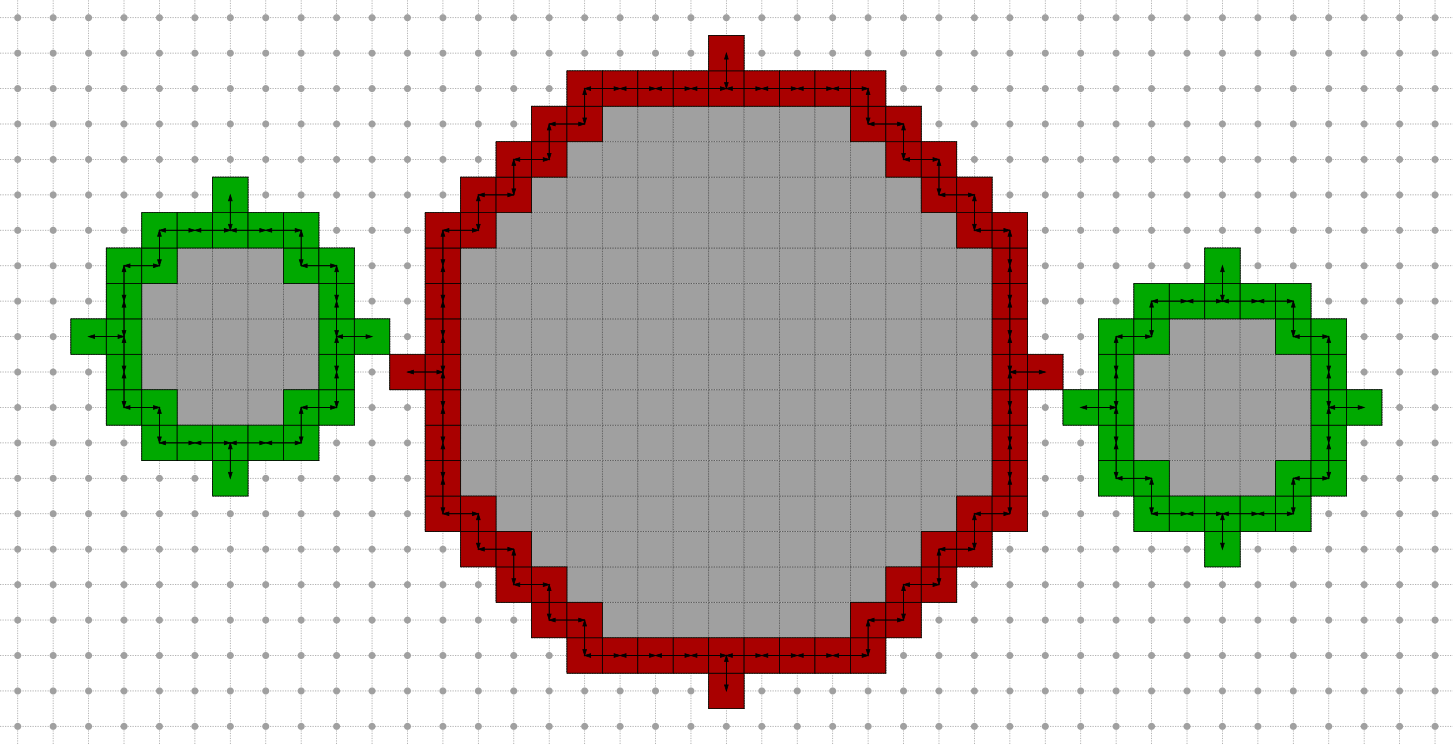
\includegraphics[width=0.48\textwidth]{bubble-object-color-borders-48}
  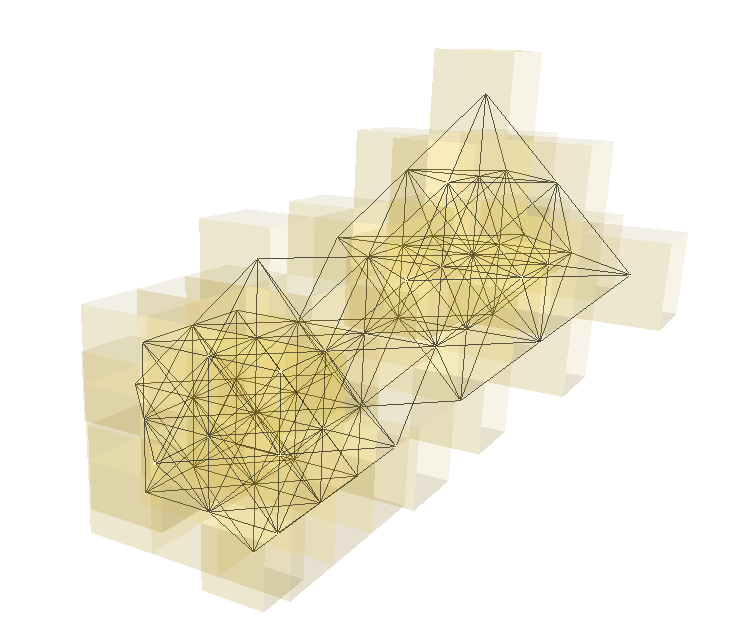
\includegraphics[width=0.48\textwidth]{object-3d-18-6}
\end{frame}
%------------------------------------------------------------------------------
\begin{frame}[fragile]
  \frametitle{Expander: digital layers in an object}
  
  \begin{itemize}
  \item Expansion layer by layer within an object, starting from an initial core
  \item core = a point or a pointset specified by iterators
  \item each new layer = the set of points of the object adjacent to
    the preceding layer
  \item each layer is iterable, has a digital distance to core
  \item finished when no more neighbor expansion is possible
  \item useful for \alert{connectedness}, \alert{geodesic
    neighborhoods} and thus \alert{simpleness}
  \end{itemize}
\end{frame}
%------------------------------------------------------------------------------

%------------------------------------------------------------------------------
\begin{frame}
  \frametitle{Expander: digital layers in an object}
  \begin{center}
    \begin{tabular}{cc}
      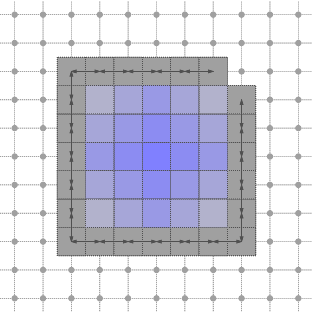
\includegraphics[width=0.4\textwidth]{house-layers4-4} &
      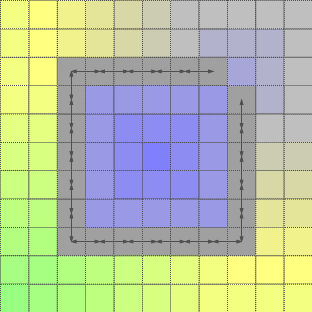
\includegraphics[width=0.4\textwidth]{house-layers4-8} \\
      background in 4-adj &
      background in 8-adj \\
    \end{tabular}

    \texttt{tests/topology/testSimpleExpander.cpp}
  \end{center}
\end{frame}

%------------------------------------------------------------------------------
\begin{frame}[fragile]
  \frametitle{Example: greedy homotopic thinning}
    \scriptsize
    \lstset{language=c++, numbers=left, tabsize=2, frame=single, breaklines=true, basicstyle=\ttfamily,
      numberstyle=\tiny\ttfamily, framexleftmargin=13mm, xleftmargin=12mm,keywordstyle=\color{blue}\bfseries,%
      commentstyle=\color{red}\textit}
    \begin{lstlisting}
  int layer = 0;
  do {
      DigitalSet & S = shape.pointSet();
      std::queue<DigitalSet::Iterator> Q;
      for ( DigitalSet::Iterator it = S.begin(); it != S.end(); ++it )
        if ( shape.\alertred{isSimple}( *it ) )
          Q.push( it );
      nb_simple = 0;
      while ( ! Q.empty() ) {
        DigitalSet::Iterator it = Q.front();
        Q.pop();
        if ( shape.isSimple( *it ) ) {
          S.erase( *it );
          ++nb_simple;
        }
      }
      ++layer;
  } while ( nb_simple != 0 );
    \end{lstlisting}
    \normalsize
    See \texttt{testObject.cpp}
\end{frame}
%------------------------------------------------------------------------------

%------------------------------------------------------------------------------
\begin{frame}[fragile]
  \frametitle{Example: greedy homotopic thinning}
  \begin{center}
    \begin{tabular}{cc}
      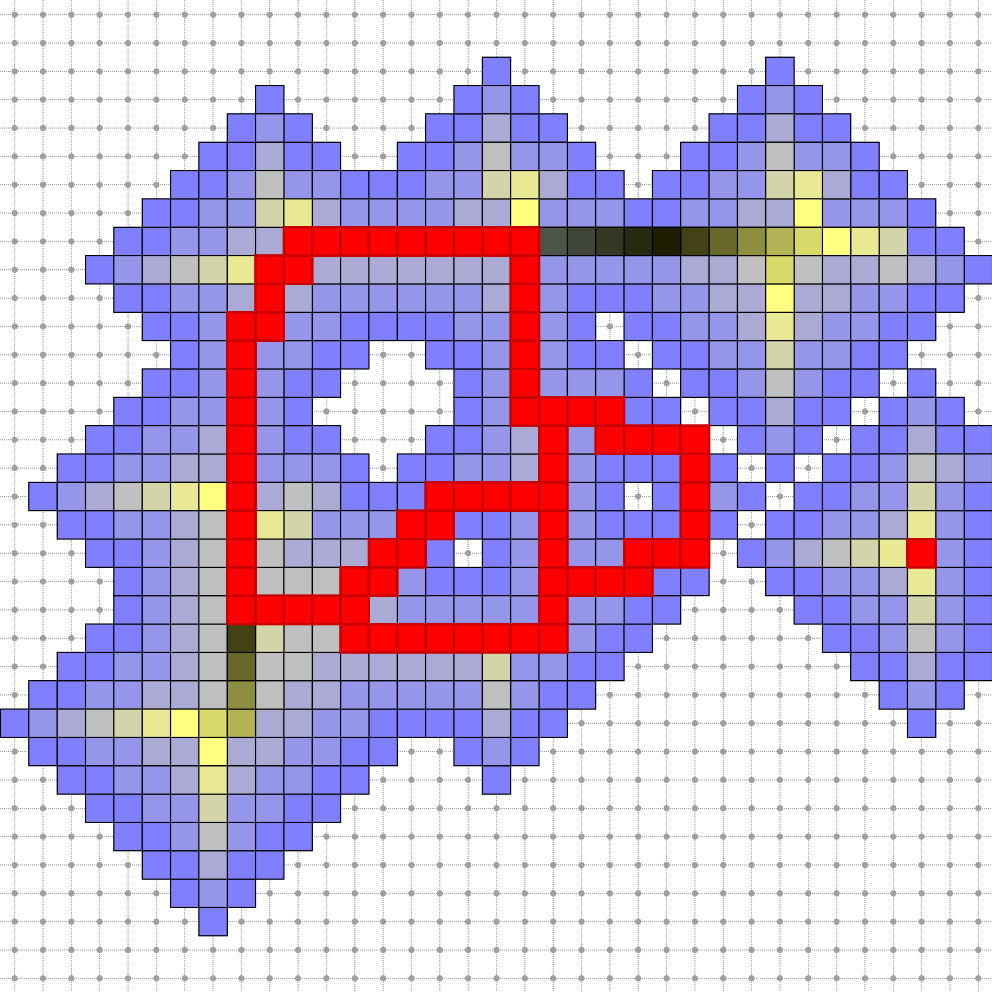
\includegraphics[width=0.4\textwidth]{shape-thinning-4-8} &
      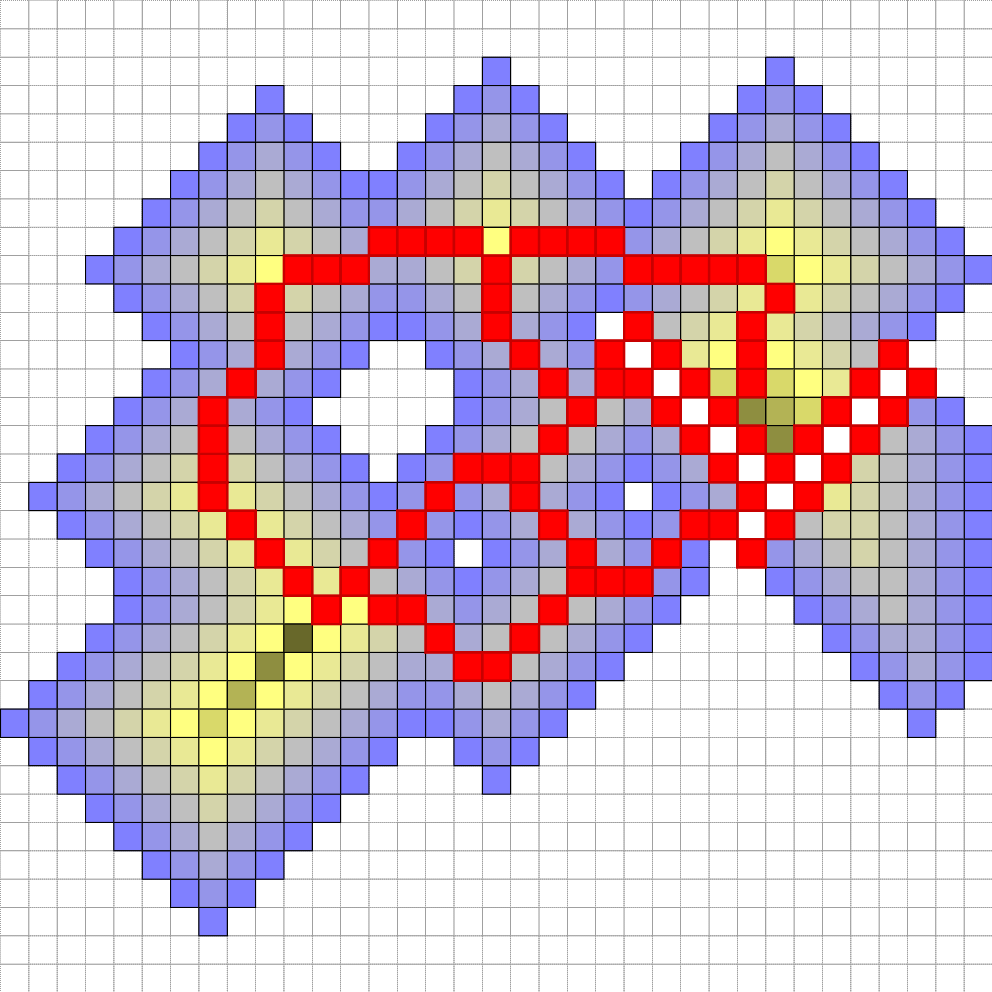
\includegraphics[width=0.4\textwidth]{shape-thinning-8-4} \\
      thinning in (4,8) &
      thinning in (8,4) \\
    \end{tabular}

    \texttt{tests/topology/testObject.cpp}
  \end{center}
\end{frame}
%------------------------------------------------------------------------------

%------------------------------------------------------------------------------
\begin{frame}
  \frametitle{Example: greedy homotopic thinning 3D}
  \begin{center}
    \begin{tabular}{c}
      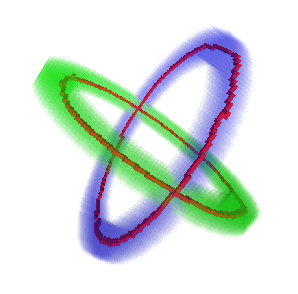
\includegraphics[width=0.55\textwidth]{thinning-3d} \\
      thinning in (6,26) \\
    \end{tabular}
    
    The thinning algorithm is the same as in 2d.
  \end{center}
\end{frame}
%------------------------------------------------------------------------------

\section{Cubical cellular topology}

%%%     \item cells, adjacent and incident cells, faces and cofaces
%%%     \item signed cells, signed incidence, 

%------------------------------------------------------------------------------
\begin{frame}
  \frametitle{Digital space as a regular cubical cell complex}

  \begin{itemize}
  \item classical combinatorial topology: cellular decomposition of
    $\R^n$ into the regular grid topology [Khalimsky,Kovalevsky]

  \item cellular complex whose cells are points, unit edges, unit squares, etc
      
  \item Khalimsky view as a cartesian product of $\Z^n$ with alternate
    topologies.

    \begin{center}
    \begin{tabular}{cc}
      \includegraphics[width=0.4\textwidth]{RegularGrid2} &
      \includegraphics[width=0.48\textwidth]{KhalimskyIsomorphism} \\
    \end{tabular}
    \end{center}

  \item even coordinate = closed, odd coordinate = open
  \end{itemize}
\end{frame}
%------------------------------------------------------------------------------

%------------------------------------------------------------------------------
\begin{frame}
  \frametitle{Model of cubical cellular space I}

  \alertred{Genericity} $\Rightarrow$ concept \Concept{CCellularGridSpaceND}

  Model \Class{KhalimskySpaceND<dim,Integer>}
  \begin{itemize}
  \item Inner types: \Class{Space}, \Class{Point}, \Class{Vector}, \ldots \\
    \Class{Cell}, \Class{SCell}, \Class{Cells}, \Class{SCells}
  \item the user provide a bounding box at space creation\\
    \Method{init}( Point, Point, bool ) returns bool
  \item cells may be signed (algebraic manipulation)
  \item cells are black boxes: managed through methods of space
  \end{itemize}
\end{frame}
%------------------------------------------------------------------------------

%------------------------------------------------------------------------------
\begin{frame}
  \frametitle{Model of cubical cellular space II}

  \begin{itemize}
  \item cells are black boxes: managed through methods of space
    \begin{itemize}
    \item creation: \Method{uCell}, \Method{sCell}, \ldots
    \item read/write access: \Method{uCoord}, \ldots 
    \item sign services: \Method{signs}, \Method{unsigns}, \Method{sOpp}, 
    \item topology services: \Method{uDim}, \Method{uIsSurfel}, \ldots
    \item direction iterators: \Method{uDirs}, \Method{uOrthDirs},  \ldots
    \item geometric services: \Method{uFirst}, \Method{uLast}, \Method{uTranslation}, \Method{uProjection}, \ldots
    \item neighborhood services: \Method{uNeighborhood}, \Method{uAdjacent}, \ldots
    \item incidence services: \Method{uIncident}, \Method{uFaces}, \ldots
    \item direct orientation service: \Method{sDirect}, \ldots
    \end{itemize}
  \end{itemize}
\end{frame}
%------------------------------------------------------------------------------

%------------------------------------------------------------------------------
\begin{frame}[fragile]
  \frametitle{Example: cell creation and view}
    \scriptsize
    \lstset{language=c++, numbers=left, tabsize=2, frame=single, breaklines=true, basicstyle=\ttfamily,
      numberstyle=\tiny\ttfamily, framexleftmargin=13mm, xleftmargin=12mm,keywordstyle=\color{blue}\bfseries,%
      commentstyle=\color{red}\textit}
    \begin{lstlisting}
 Viewer3D viewer;
 ...
 KSpace K;
 Point plow(0,0,0);  
 Point pup(3,3,2);
 // should return true
 K.init( plow, pup, true );
 // Drawing cell of dimension 3
 Cell voxelA = K.uCell(Point(1,1,1));
 SCell voxelB = K.sCell(Point(1,1,3));
 viewer << voxelB << voxelA;
 // drawing cells of dimension 2
 SCell surfelA = K.sCell( Point( 2, 1, 3 ) ); 
 SCell surfelB = K.sCell( Point( 1, 0, 1 ), false ); 
 Cell surfelC = K.uCell( Point( 1, 2, 1 ) ); 
 SCell surfelD = K.sCell( Point( 1, 1, 0 ) );
 Cell surfelE = K.uCell( Point( 1, 1, 2 ) ); 
 viewer << surfelA << surfelB << surfelC << surfelD << surfelE;
    \end{lstlisting}
    \normalsize
\end{frame}
%------------------------------------------------------------------------------

%------------------------------------------------------------------------------
\begin{frame}
  \frametitle{Visualization of cells in 2D/3D}

  You can put cells in a 2D/3D visualization stream.
  \begin{tabular}{cc}
  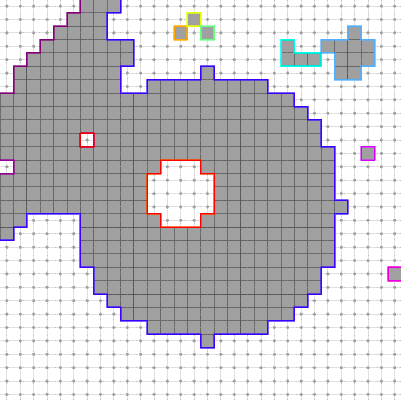
\includegraphics[width=0.4\textwidth]{fcExtraction1}&
  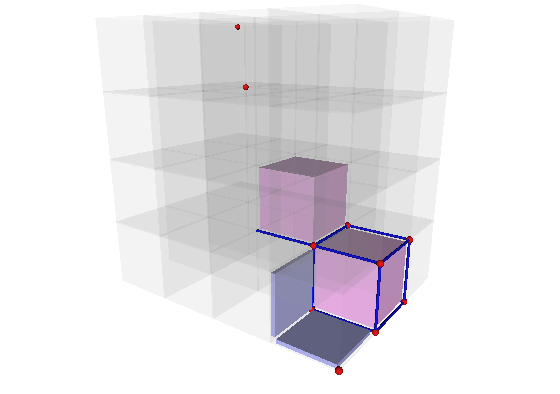
\includegraphics[width=0.47\textwidth]{3DKhalimskyCells}\\
  \end{tabular}
  
\end{frame}
%------------------------------------------------------------------------------

%------------------------------------------------------------------------------
\begin{frame}
  \frametitle{Why signing cells: algebraic view}

  \begin{itemize}

  \item<1-> {\em $r$-chain} : formal sum of $r$-cells
    \only<1>{
      \begin{itemize}
	
      \item Example : $\sum_i +o^n_i$, with $o^n_i$ $n$-cells, is a
        digital object
	      
      \item Example : $\sum_i a_j s^{n-1}_j$, with $s^{n-1}_j$
	$n-1$-cells, is a digital surface
	      
      \end{itemize}
	    
      \begin{columns}
	\column{0.4\textwidth}
	\begin{tabular}{r}
	  {spels \color{green}{$+o^n_i$}} \\ 
	  {surfels \color{blue}{$+s^{n-1}_j$}} \\
	  {and \color{magenta}{$-s^{n-1}_j$}}
	\end{tabular}
	\column{0.4\textwidth}
	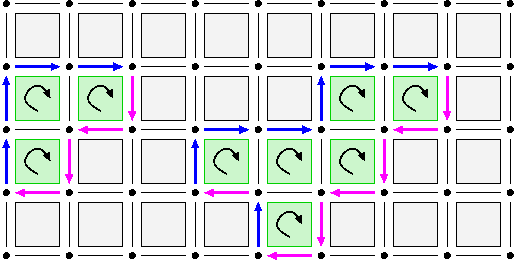
\includegraphics[width=\textwidth]{Boundaries}
      \end{columns}
    }

  \item<2-> Linear operators \alert<2>{boundary $\Delta$} and
    \alert<2>{co-boundary $\nabla$}
    
    \only<2->{
      \begin{itemize}
      \item $\Delta$ : $r$-chain $\mapsto$ $r-1$-chain ($\equiv$ (low) incidence)
      \item $\nabla$: $r$-chain $\mapsto$ $r+1$-chain ($\equiv$ (up) incidence)
      \item $\Delta \Delta = 0$ and $\nabla \nabla = 0$ (Homology)
      \end{itemize}
    }
    \only<2-7>{
      \begin{columns}[c]
	\column{0.3\textwidth}
        
	\begin{flushright}
	  {$\Delta$ {\color{green}{$\sum +o^n_i$}} ? }
	\end{flushright}
        
	\column{0.5\textwidth}
	\only<2>{
	  \includegraphics[width=\textwidth]{BdryOp-1}
	}
	\only<3>{
	    \includegraphics[width=\textwidth]{BdryOp-2}
	}
	\only<4>{
	  \includegraphics[width=\textwidth]{BdryOp-3}
	}
	\only<5>{
	  \includegraphics[width=\textwidth]{BdryOp-4}
	}
	\only<6>{
	  \includegraphics[width=\textwidth]{BdryOp-5}
	}
	\only<7>{
	  \includegraphics[width=\textwidth]{BdryOp-6}
	}
      \end{columns}
    }
  \item<8-> coefficients are generally taken $\pm 1$. It is enough to
    sign cells to design that kind of operators.
  \end{itemize}

\end{frame}

%------------------------------------------------------------------------------
\begin{frame}
  \frametitle{Applications}

  \begin{enumerate}
    \item<1-> Any object boundary is closed.

      \only<1>{
        Boundary of a digital object $O$ = $\Delta O$
        
        \begin{columns}[c]
          \column{0.5\textwidth}
          \begin{flushright}
            \includegraphics[width=0.6\textwidth]{fig-boundary}
          \end{flushright}
          \column{0.5\textwidth} 
          \begin{block}{$\partial O$ is a closed surface.}
            Since $\Delta \Delta = 0$, the boundary of a digital object is
            a surface without boundary.
          \end{block}
        \end{columns}
      }
      \item<2-> Neighborhood and tracking over $\partial O$

        \only<2>{
          \begin{itemize}
          \item Any surfel has $2n-2$ neighbors
          \item Formal definition of the two neighbors of a surfel
            $\sigma$, of orth. dir. $i$, along direction $j \neq i$.
            
            $\Delta^{\epsilon}_i \nabla^{\mu}_j \sigma$,
            $\nabla^{\epsilon}_i \Delta^{\epsilon}_i \sigma$,
            $\Delta^{\epsilon}_i \nabla^{-\mu}_j \sigma$ with $\mu =
            \pm 1$ and $\epsilon = \pm 1$
            
            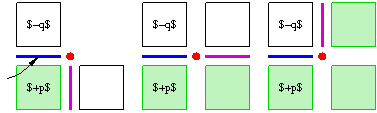
\includegraphics[height=1.5cm]{IntAdjacency}
            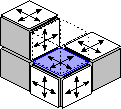
\includegraphics[height=1.5cm]{SurfaceTracking2}
            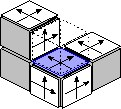
\includegraphics[height=1.5cm]{SurfaceTracking}
            
          \item Neighbors are oriented (\alertred{direct} or
            \alertred{indirect} orientation)
          \end{itemize}
        }

  \end{enumerate}
\end{frame}
%------------------------------------------------------------------------------

\section{Digital surface topology}

%------------------------------------------------------------------------------
\begin{frame}[fragile]
  \frametitle{Adjacency between surfels}
  \begin{itemize}
  \item \Class{SurfelAdjacency<dim>} specifies interior toward
    exterior or the reverse for each direction.
    \scriptsize
    \lstset{language=c++, numbers=left, tabsize=2, frame=single, breaklines=true, basicstyle=\ttfamily,
      numberstyle=\tiny\ttfamily, framexleftmargin=13mm, xleftmargin=12mm,keywordstyle=\color{blue}\bfseries,%
      commentstyle=\color{red}\textit}
    \begin{lstlisting}
SurfelAdjacency<2> sAdj1( true ); // (4,8) 
SurfelAdjacency<2> sAdj2( false ); // (8,4)
SurfelAdjacency<3> sAdj3( true ); // (6,18)
SurfelAdjacency<3> sAdj4( false ); // (18,6)
sAdj4.setAdjacency( 0, 1, true ); // hybrid 
    \end{lstlisting}
    \normalsize
  \item \Class{SurfelNeighborhood<KSpace>} computes adjacent surfels
    \begin{itemize}
    \item initialized by \Method{init( KSpace*, SurfelAdjacency<dim>, Cell )}
    \item surfel can be changed \Method{setSurfel}
    \item get surrounding spels: \Method{innerSpel}(), \Method{innerAdjacentSpel}( Dimension, bool ), \ldots
    \item get following surfels: \Method{follower1}( Dimension, bool )
    \item get adjacent surfels: \Method{getAdjacentOnSpelSet}, \ldots
    \end{itemize}
  \end{itemize}
\end{frame}
%------------------------------------------------------------------------------

%------------------------------------------------------------------------------
\begin{frame}[fragile]
  \frametitle{Tracking surfels through surfel adjacencies I}

  \scriptsize
  \Class{Surfaces<KSpace>}.\Method{trackClosedBoundary}( 
  \begin{itemize}
    \item SCellSet \& surface, 
    \item const KSpace \& K,
    \item const SurfelAdjacency<KSpace::dimension> \& surfel\_adj,
    \item const PointPredicate \& pp, 
    \item const SCell \& start\_surfel )
  \end{itemize}

  \begin{center}
    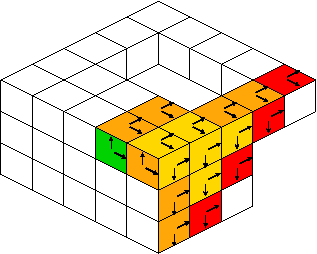
\includegraphics[width=0.4\textwidth]{suivi-artzy}
  \end{center}
\end{frame}
%------------------------------------------------------------------------------

%------------------------------------------------------------------------------
\begin{frame}[fragile]
  \frametitle{}

  \scriptsize
    \lstset{language=c++, numbers=left, tabsize=2, frame=single, breaklines=true, basicstyle=\ttfamily,
      numberstyle=\tiny\ttfamily, framexleftmargin=13mm, xleftmargin=12mm,keywordstyle=\color{blue}\bfseries,%
      commentstyle=\color{red}\textit}
    \begin{lstlisting}
SCell b;  // current surfel
SCell bn; // neighboring surfel
SurfelNeighborhood<KSpace> SN;
SN.init( &K, &surfel_adj, start_surfel );
std::queue<SCell> qbels;
qbels.push( start_surfel );
surface.insert( start_surfel ); // output
while ( ! qbels.empty() ) { // For all pending bels
  b = qbels.front();
  qbels.pop();
  SN.setSurfel( b );
  for ( DirIterator q = K.sDirs( b ); q != 0; ++q ) {
    Dimension track_dir = *q;
    // One pass, look for direct orientation
    if ( SN.getAdjacentOnPointPredicate( bn, pp, track_dir, K.sDirect( b, track_dir ) ) )
    {
      if ( surface.find( bn ) == surface.end() )
      {
        surface.insert( bn );
        qbels.push( bn );
      }
    }
  } // end for 
} // end while 
    \end{lstlisting}
  \normalsize
\end{frame}
%------------------------------------------------------------------------------

%------------------------------------------------------------------------------
\begin{frame}[fragile]
  \frametitle{Helper class Surfaces}

  Provide methods for
  \begin{itemize}
  \item finding a bel (i.e. a surfel between inside/outside of object)
  \item track boundaries in $n$D (closed or not)
  \item track contours of 2D shapes
  \item track 2D slices of $n$ shapes
  \item extract all contours of a 2D domain
  \item extract all boundaries of a $n$D shape
  \item computes the whole boundary of a $n$D shape by scanning
  \end{itemize}

  (with B. Kerautret)

\end{frame}
%------------------------------------------------------------------------------

%------------------------------------------------------------------------------
\begin{frame}[fragile]
  \frametitle{Surface tracking example}

  \begin{center}
    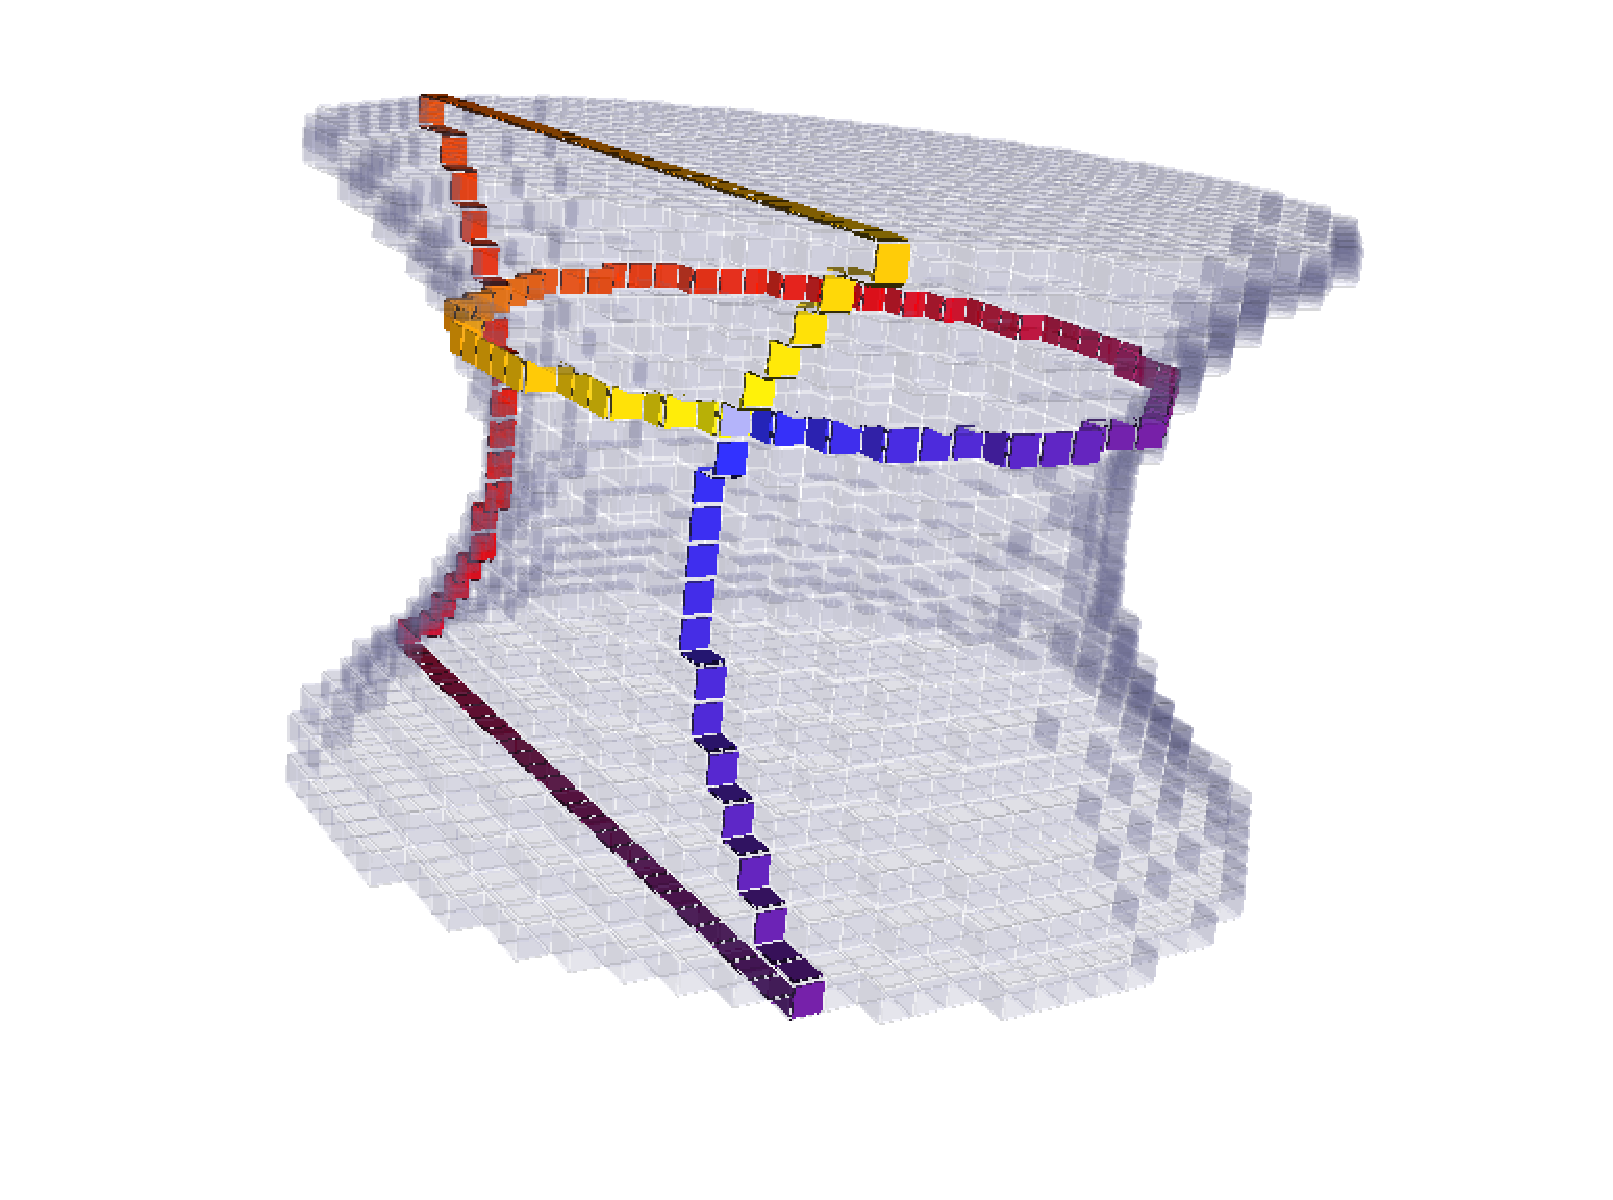
\includegraphics[width=0.8\textwidth]{surfelTracking}
  \end{center}

\end{frame}
%------------------------------------------------------------------------------

%------------------------------------------------------------------------------
\begin{frame}[fragile]
  \frametitle{Surface tracking snippet}

  \scriptsize
  \lstset{language=c++, numbers=left, tabsize=2, frame=single, breaklines=true, basicstyle=\ttfamily,
    numberstyle=\tiny\ttfamily, framexleftmargin=13mm, xleftmargin=12mm,keywordstyle=\color{blue}\bfseries,%
    commentstyle=\color{red}\textit}
  \begin{lstlisting}
  // Extract an initial boundary cell
  Z3i::SCell aCell = Surfaces<Z3i::KSpace>::findABel(ks, set3dPredicate);
  // Extracting all boundary surfels connected to the initial one
  Surfaces<Z3i::KSpace>::trackBoundary( vectBdrySCellALL, ks,SAdj, set3dPredicate, aCell );
    
  // Extract the boundary contour associated to the initial surfel in its first direction
  Surfaces<Z3i::KSpace>::track2DBoundary( vectBdrySCell, ks, *(ks.sDirs( aCell )), SAdj, set3dPredicate, aCell );
  
  // Extract the bondary contour associated to the initial surfel in its second direction
  Surfaces<Z3i::KSpace>::track2DBoundary( vectBdrySCell2, ks, *(++(ks.sDirs( aCell ))), SAdj, set3dPredicate, aCell );  
  \end{lstlisting}
\end{frame}

%------------------------------------------------------------------------------
\begin{frame}[fragile]
  \frametitle{Getting the contour of a digitized shape}

  \scriptsize
  \lstset{language=c++, numbers=left, tabsize=2, frame=single, breaklines=true, basicstyle=\ttfamily,
    numberstyle=\tiny\ttfamily, framexleftmargin=13mm, xleftmargin=12mm,keywordstyle=\color{blue}\bfseries,%
    commentstyle=\color{red}\textit}
  \begin{lstlisting}
  // Digitizer
  GaussDigitizer<Space,Shape> dig;  
  dig.attach( aShape ); // attaches the shape.
  Vector vlow(-1,-1); Vector vup(1,1);
  dig.init( aShape.getLowerBound()+vlow, aShape.getUpperBound()+vup, h ); 
  Domain domain = dig.getDomain();
  // Extracts shape boundary
  SurfelAdjacency<KSpace::dimension> SAdj( true );
  SCell bel = Surfaces<KSpace>::findABel( K, dig, 10000 );
  // Getting the consecutive surfels of the 2D boundary
  std::vector<Point> points;
  Surfaces<KSpace>::track2DBoundaryPoints( points, K, SAdj, dig, bel );
  // Create GridCurve
  GridCurve<KSpace> gridcurve;
  gridcurve.initFromVector( points );
  \end{lstlisting}
\end{frame}

%% %------------------------------------------------------------------------------
%% \begin{frame}
%%   \frametitle{Conclusion and perspectives}
  
%%   \begin{itemize}
%%   \item complete Rosenfeld's approach: curves and separation
%%   \item whole digital topology framework of Herman and Udupa
%%     \begin{itemize}
%%     \item digital surface as a couple of $\omega$-adjacent points
%%     \item immediate interior and exterior, interior and exterior
%%     \item $\kappa \lambda$-borders, $\kappa \lambda$-boundaries
%%     \item digital pictures
%%     \end{itemize}
%%   \item interpixel topology or cartesian cellular grid topology 
%%   \end{itemize}
%%   See on-line doc.: \Cb{Digital topology and digital objects}

%% \end{frame}
%% %------------------------------------------------------------------------------

%------------------------------------------------------------------------------
\begin{frame}%[allowframebreaks]
  \frametitle{To go further}

  On-line user guide in DGtal documentation
  \begin{itemize}
  \item Topology Package
    \begin{itemize}
    \item Digital topology and digital objects
    \item Cellular grid space and topology, cells, digital surfaces\\
    \end{itemize}
  \end{itemize}
  (nicely illustration in 3D, thanks to B. Kerautret)
\end{frame}


%------------------------------------------------------------------------------
\begin{frame}%[allowframebreaks]
  \frametitle{Next objectives}

  \begin{enumerate}
  \item classical digital topology
    \begin{itemize}
    \item other adjacencies
    \item Adjacency = unoriented graph, create associated concepts
    \item make everything faster with specialization (especially
      simpleness)
    \end{itemize}
  \item cubical cellular topology
    \begin{itemize}
    \item cubical complexes, interior, closure
    \item path, mapping (homotopy) 
    \item chains, boundary operator, cochains, coboundary
    \item (co)homology
    \end{itemize}
  \item digital surface topology
    \begin{itemize}
    \item digital surface concept, digital surface graph and
      cograph, digital surface map
    \end{itemize}
  \end{enumerate}
\end{frame}
%------------------------------------------------------------------------------

%%% %------------------------------------------------------------------------------
%%% \begin{frame}[fragile]
%%%   \frametitle{Insight into signed cell mechanism}

%%%   \scriptsize
%%%   \Class{SurfelNeighborhood<KSpace>}.\Method{getAdjacentOnDigitalSet}( SCell \& adj\_surfel, const DigitalSet \& obj, Dimension track\_dir, bool pos )

%%%   \lstset{language=c++, numbers=left, tabsize=2, frame=single, breaklines=true, basicstyle=\ttfamily,
%%%     numberstyle=\tiny\ttfamily, framexleftmargin=13mm, xleftmargin=12mm,keywordstyle=\color{blue}\bfseries,%
%%%     commentstyle=\color{red}\textit}
%%%   \begin{lstlisting}
%%%   Point inner_spel_pt = mySpace->sCoords(innerSpel());
%%%   ...
%%%   // Check type of surfel adjacency.
%%%   if ( mySurfelAdj->getAdjacency(orthDir(), track_dir))
%%%     { // interior to exterior. Check first next bel.
%%%       if ( obj.find( mySpace->sCoords( innerAdjacentSpel( track_dir, pos ) ) ) == obj.end() )
%%%         adj_surfel = follower1( track_dir, pos );
%%%       // Check second next bel.
%%%       else if ( obj.find( mySpace->sCoords( outerAdjacentSpel( track_dir, pos ) ) ) == obj.end() )
%%%         adj_surfel = follower2( track_dir, pos ); 
%%%       else // The third one is then the right one.
%%%         adj_surfel = follower3( track_dir, pos ); 
%%%     }
%%%   \end{lstlisting}
%%%   \normalsize
%%% \end{frame}


\end{document}
